\documentclass{beamer}
\usepackage[utf8]{inputenc}
\usepackage[T1]{fontenc}
\usepackage{graphicx}
\usepackage{xcolor}
\usepackage{listings}
\usepackage{tikz}
\usepackage{amsmath}
\usepackage{hyperref}

% Theme
\usetheme{Madrid}
\usecolortheme{default}

% Colors
\definecolor{codeblue}{RGB}{0,102,204}
\definecolor{codegray}{RGB}{128,128,128}
\definecolor{codegreen}{RGB}{0,128,0}
\definecolor{backcolour}{RGB}{245,245,245}

% Code listing style
\lstdefinestyle{cstyle}{
    backgroundcolor=\color{backcolour},
    commentstyle=\color{codegreen},
    keywordstyle=\color{codeblue},
    numberstyle=\tiny\color{codegray},
    stringstyle=\color{red},
    basicstyle=\ttfamily\footnotesize,
    breakatwhitespace=false,
    breaklines=true,
    keepspaces=true,
    numbers=left,
    numbersep=5pt,
    showspaces=false,
    showstringspaces=false,
    showtabs=false,
    tabsize=2,
    frame=single
}

\lstset{style=cstyle}

% Title page info
\title{Day 3: Memory Management and Data Structures}
\subtitle{C Programming for Post-Silicon Validation Engineers}
\author{Course Instructor}
\date{6-Day Intensive Bootcamp}
\institute{Post-Silicon Validation Training Program}

\begin{document}

\frame{\titlepage}

\begin{frame}
\frametitle{Welcome to Day 3!}
\begin{center}
\Large The Most Important Day: Pointers and Memory
\end{center}

\begin{itemize}
    \item \textbf{Yesterday:} Control flow and debugging mastery
    \item \textbf{Today's Mission:} Conquer pointers and memory management
    \item \textbf{Validation Focus:} Direct register access and chip modeling
    \item \textbf{New Addition:} AI coding assistants introduction
    \item \textbf{Outcome:} Complete chip state monitoring system!
\end{itemize}

\vspace{0.5cm}
\begin{center}
\textit{"Understanding pointers is the key to mastering C"} - Every C programmer ever
\end{center}
\end{frame}

\begin{frame}
\frametitle{Today's Learning Objectives}
By the end of Day 3, you will:

\begin{enumerate}
    \item Understand pointers and memory addressing
    \item Master array manipulation and string handling
    \item Create structures to model hardware components
    \item Perform bit manipulation for register operations
    \item Use AI tools responsibly for code assistance
    \item Build comprehensive chip validation systems
\end{enumerate}

\vspace{0.5cm}
\begin{alertblock}{Critical Day}
Today's concepts are fundamental to embedded programming!
\end{alertblock}
\end{frame}

\begin{frame}
\frametitle{Memory: The Foundation}
\begin{center}
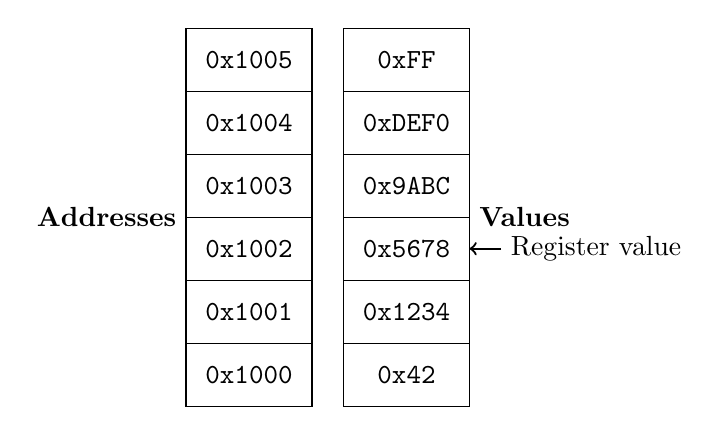
\begin{tikzpicture}[scale=0.8]
% Memory blocks
\foreach \i in {0,1,2,3,4,5} {
    \draw (0,\i) rectangle (2,\i+1);
    \node at (1,\i+0.5) {\texttt{0x100\i}};
    \draw (2.5,\i) rectangle (4.5,\i+1);
}

% Values
\node at (3.5,0.5) {\texttt{0x42}};
\node at (3.5,1.5) {\texttt{0x1234}};
\node at (3.5,2.5) {\texttt{0x5678}};
\node at (3.5,3.5) {\texttt{0x9ABC}};
\node at (3.5,4.5) {\texttt{0xDEF0}};
\node at (3.5,5.5) {\texttt{0xFF}};

% Labels
\node[left] at (0,3) {\textbf{Addresses}};
\node[right] at (4.5,3) {\textbf{Values}};

% Arrow pointing to specific location
\draw[thick,->] (5,2.5) -- (4.5,2.5);
\node[right] at (5,2.5) {Register value};
\end{tikzpicture}
\end{center}

\textbf{Key concepts:}
\begin{itemize}
    \item Every variable has an address in memory
    \item Addresses are just numbers (like 0x1002)
    \item We can store and manipulate these addresses
    \item This is exactly how hardware registers work!
\end{itemize}
\end{frame}

\begin{frame}[fragile]
\frametitle{Pointers: Your Gateway to Hardware}
\begin{lstlisting}[language=C]
#include <stdio.h>

int main() {
    int voltage = 3300;  // 3.3V in millivolts
    int *voltage_ptr;    // Pointer to an integer

    voltage_ptr = &voltage;  // Get address of voltage

    printf("Value: %d mV\n", voltage);
    printf("Address: %p\n", (void*)&voltage);
    printf("Pointer holds: %p\n", (void*)voltage_ptr);
    printf("Value via pointer: %d mV\n", *voltage_ptr);

    // Modify through pointer (like writing to register)
    *voltage_ptr = 5000;  // Change to 5.0V
    printf("New value: %d mV\n", voltage);

    return 0;
}
\end{lstlisting}
\end{frame}

\begin{frame}
\frametitle{Pointer Syntax Breakdown}
\begin{center}
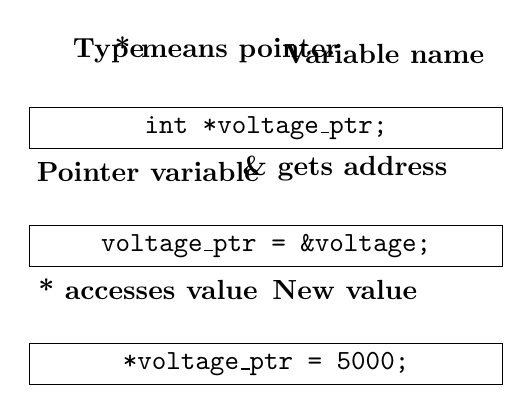
\begin{tikzpicture}
% Declaration
\node[draw, rectangle, minimum width=6cm] at (0,3) {\texttt{int *voltage\_ptr;}};
\node[above] at (-2,3.7) {\textbf{Type}};
\node[above] at (-0.5,3.7) {\textbf{* means pointer}};
\node[above] at (1.5,3.7) {\textbf{Variable name}};

% Assignment
\node[draw, rectangle, minimum width=6cm] at (0,1.5) {\texttt{voltage\_ptr = \&voltage;}};
\node[above] at (-1.5,2.2) {\textbf{Pointer variable}};
\node[above] at (1,2.2) {\textbf{\& gets address}};

% Dereferencing
\node[draw, rectangle, minimum width=6cm] at (0,0) {\texttt{*voltage\_ptr = 5000;}};
\node[above] at (-1.5,0.7) {\textbf{* accesses value}};
\node[above] at (1,0.7) {\textbf{New value}};
\end{tikzpicture}
\end{center}

\vspace{0.5cm}
\textbf{Memory mantra:}
\begin{itemize}
    \item \texttt{\&} = "address of"
    \item \texttt{*} = "value at" (when used with pointer)
    \item \texttt{*} = "pointer to" (when declaring)
\end{itemize}
\end{frame}

\begin{frame}[fragile]
\frametitle{Pointers in Hardware Validation}
\begin{lstlisting}[language=C]
#include <stdio.h>
#include <stdint.h>

// Simulate memory-mapped register access
#define CONTROL_REG_ADDR  0x40000000
#define STATUS_REG_ADDR   0x40000004

// In real embedded code, these would be:
// volatile uint32_t *control_reg = (uint32_t*)CONTROL_REG_ADDR;
// volatile uint32_t *status_reg = (uint32_t*)STATUS_REG_ADDR;

// For simulation, use regular variables
uint32_t control_register = 0x0000;
uint32_t status_register = 0x0001;

void write_control_register(uint32_t value) {
    uint32_t *reg_ptr = &control_register;
    *reg_ptr = value;
    printf("Control register set to: 0x%08X\n", value);
}

uint32_t read_status_register(void) {
    uint32_t *reg_ptr = &status_register;
    return *reg_ptr;
}
\end{lstlisting}
\end{frame}

\begin{frame}[fragile]
\frametitle{Arrays: Collections of Data}
\begin{lstlisting}[language=C]
#include <stdio.h>

int main() {
    // Array of register values
    int registers[8] = {0x1000, 0x2000, 0x3000, 0x4000,
                        0x5000, 0x6000, 0x7000, 0x8000};

    // Access elements
    printf("First register: 0x%04X\n", registers[0]);
    printf("Last register: 0x%04X\n", registers[7]);

    // Loop through all registers
    for (int i = 0; i < 8; i++) {
        printf("Register[%d]: 0x%04X\n", i, registers[i]);
    }

    // Modify register value
    registers[3] = 0x9999;
    printf("Modified register[3]: 0x%04X\n", registers[3]);

    return 0;
}
\end{lstlisting}

\textbf{Array facts:}
\begin{itemize}
    \item Arrays are stored in contiguous memory
    \item Array name is a pointer to first element
    \item \texttt{registers[i]} is same as \texttt{*(registers + i)}
\end{itemize}
\end{frame}

\begin{frame}[fragile]
\frametitle{Strings: Arrays of Characters}
\begin{lstlisting}[language=C]
#include <stdio.h>
#include <string.h>

int main() {
    // Different ways to declare strings
    char chip_id[] = "RP2040";
    char test_result[10];
    char *status_msg = "PASS";

    // String operations
    strcpy(test_result, "FAIL");
    printf("Chip ID: %s\n", chip_id);
    printf("Test Result: %s\n", test_result);
    printf("Status: %s\n", status_msg);

    // String comparison for validation
    if (strcmp(test_result, "PASS") == 0) {
        printf("Validation successful!\n");
    } else {
        printf("Validation failed!\n");
    }

    return 0;
}
\end{lstlisting}
\end{frame}

\begin{frame}[fragile]
\frametitle{Structures: Modeling Hardware Components}
\begin{lstlisting}[language=C]
#include <stdio.h>
#include <stdint.h>

// Structure to represent a chip's state
typedef struct {
    uint32_t control_reg;
    uint32_t status_reg;
    uint32_t error_reg;
    char chip_id[16];
    float temperature;
    int test_count;
} ChipState;

int main() {
    ChipState chip1;

    // Initialize chip state
    chip1.control_reg = 0x12345678;
    chip1.status_reg = 0x00000001;
    chip1.error_reg = 0x00000000;
    strcpy(chip1.chip_id, "RP2040-001");
    chip1.temperature = 45.5;
    chip1.test_count = 0;

    printf("Chip: %s\n", chip1.chip_id);
    printf("Temperature: %.1fC\n", chip1.temperature);
    printf("Status: 0x%08X\n", chip1.status_reg);

    return 0;
}
\end{lstlisting}
\end{frame}

\begin{frame}
\frametitle{Structure Benefits for Validation}
\textbf{Why use structures?}
\begin{itemize}
    \item \textbf{Organization:} Group related data together
    \item \textbf{Clarity:} \texttt{chip.temperature} vs \texttt{temp\_var\_3}
    \item \textbf{Maintainability:} Easy to add new fields
    \item \textbf{Reusability:} Same structure for multiple chips
    \item \textbf{Real-world modeling:} Matches hardware organization
\end{itemize}

\vspace{0.5cm}
\textbf{Validation applications:}
\begin{itemize}
    \item Chip state monitoring
    \item Test result collections
    \item Configuration parameters
    \item Error logging structures
    \item Multi-device management
\end{itemize}
\end{frame}

\begin{frame}[fragile]
\frametitle{Bit Manipulation: Register Control}
\begin{lstlisting}[language=C]
#include <stdio.h>
#include <stdint.h>

// Bit manipulation macros
#define SET_BIT(reg, bit)     ((reg) |= (1U << (bit)))
#define CLEAR_BIT(reg, bit)   ((reg) &= ~(1U << (bit)))
#define TOGGLE_BIT(reg, bit)  ((reg) ^= (1U << (bit)))
#define CHECK_BIT(reg, bit)   (((reg) >> (bit)) & 1U)

int main() {
    uint32_t control_reg = 0x00000000;

    printf("Initial: 0x%08X\n", control_reg);

    // Set enable bit (bit 0)
    SET_BIT(control_reg, 0);
    printf("After SET bit 0: 0x%08X\n", control_reg);

    // Set clock enable (bit 1)
    SET_BIT(control_reg, 1);
    printf("After SET bit 1: 0x%08X\n", control_reg);

    // Check if bit is set
    if (CHECK_BIT(control_reg, 0)) {
        printf("System is enabled\n");
    }

    return 0;
}
\end{lstlisting}
\end{frame}

\begin{frame}
\frametitle{Bit Operations Cheat Sheet}
\begin{center}
\begin{tabular}{|l|l|l|}
\hline
\textbf{Operation} & \textbf{Code} & \textbf{Purpose} \\
\hline
Set bit & \texttt{reg |= (1 << n)} & Turn on bit n \\
Clear bit & \texttt{reg \&= \textasciitilde(1 << n)} & Turn off bit n \\
Toggle bit & \texttt{reg \textasciicircum= (1 << n)} & Flip bit n \\
Check bit & \texttt{(reg >> n) \& 1} & Test if bit n is set \\
\hline
\end{tabular}
\end{center}

\vspace{0.5cm}
\textbf{Common validation patterns:}
\begin{itemize}
    \item \textbf{Enable/Disable:} Set control bits
    \item \textbf{Status Check:} Read status bits
    \item \textbf{Error Flags:} Check error bits
    \item \textbf{Configuration:} Set multiple bits at once
\end{itemize}

\vspace{0.5cm}
\begin{exampleblock}{Real Example}
\texttt{if (CHECK\_BIT(status\_reg, 7)) \{ /* Ready bit set */ \}}
\end{exampleblock}
\end{frame}

\begin{frame}[fragile]
\frametitle{Complete Chip Validation Example}
\begin{lstlisting}[language=C, basicstyle=\tiny]
#include <stdio.h>
#include <stdint.h>
#include <string.h>

typedef struct {
    uint32_t control_reg;
    uint32_t status_reg;
    uint32_t error_reg;
    char chip_id[16];
    float temperature;
} ChipState;

#define SET_BIT(reg, bit)    ((reg) |= (1U << (bit)))
#define CHECK_BIT(reg, bit)  (((reg) >> (bit)) & 1U)

void print_chip_status(ChipState *chip) {
    printf("\n--- Chip Status: %s ---\n", chip->chip_id);
    printf("Temperature: %.1fC\n", chip->temperature);
    printf("Control: 0x%08X\n", chip->control_reg);
    printf("Status:  0x%08X\n", chip->status_reg);
    printf("Errors:  0x%08X\n", chip->error_reg);

    // Decode status bits
    printf("Power: %s\n", CHECK_BIT(chip->status_reg, 0) ? "ON" : "OFF");
    printf("Clock: %s\n", CHECK_BIT(chip->status_reg, 1) ? "LOCKED" : "FREE");
    printf("Ready: %s\n", CHECK_BIT(chip->status_reg, 7) ? "YES" : "NO");
}

int validate_chip(ChipState *chip) {
    int errors = 0;

    if (chip->temperature > 85.0) {
        printf("ERROR: Temperature too high!\n");
        errors++;
    }

    if (!CHECK_BIT(chip->status_reg, 0)) {
        printf("ERROR: Power not enabled!\n");
        errors++;
    }

    return errors;
}
\end{lstlisting}
\end{frame}

\begin{frame}
\frametitle{Memory Safety: Common Pitfalls}
\begin{alertblock}{Dangerous Mistakes}
\begin{enumerate}
    \item \textbf{Null Pointer Dereference:} \texttt{*ptr} when \texttt{ptr == NULL}
    \item \textbf{Uninitialized Pointers:} Using pointer before assignment
    \item \textbf{Array Bounds:} Accessing \texttt{array[10]} when size is 10
    \item \textbf{Dangling Pointers:} Pointer to freed/invalid memory
    \item \textbf{Memory Leaks:} Forgetting to free allocated memory
\end{enumerate}
\end{alertblock}

\vspace{0.5cm}
\textbf{Safety practices:}
\begin{itemize}
    \item Always check pointers before use: \texttt{if (ptr != NULL)}
    \item Initialize pointers: \texttt{int *ptr = NULL;}
    \item Use array bounds checking
    \item Use tools like Valgrind for memory debugging
\end{itemize}
\end{frame}

\begin{frame}
\frametitle{AI Tools Introduction}
\begin{center}
\Large Welcome to the AI-Assisted Era!
\end{center}

\textbf{Starting today, you can use AI tools like:}
\begin{itemize}
    \item GitHub Copilot
    \item ChatGPT/GPT-4
    \item Claude
    \item Grok
\end{itemize}

\vspace{0.5cm}
\textbf{BUT with important rules:}
\begin{enumerate}
    \item \textbf{Document usage:} Always note when AI helped
    \item \textbf{Understand code:} Don't just copy-paste
    \item \textbf{Verify results:} AI can make mistakes
    \item \textbf{Learn fundamentals:} AI assists, doesn't replace learning
\end{enumerate}
\end{frame}

\begin{frame}[fragile]
\frametitle{AI Tool Evaluation Exercise}
\textbf{Let's try this together:}

\begin{enumerate}
    \item Ask AI: "Write a C function to validate voltage range"
    \item Examine the generated code
    \item Identify good and bad aspects
    \item Improve the code
    \item Document your evaluation
\end{enumerate}

\vspace{0.5cm}
\textbf{Example AI prompt:}
\begin{verbatim}
"Write a C function that takes a voltage value and
checks if it's within a valid range of 1.8V to 3.6V.
Return 1 for valid, 0 for invalid."
\end{verbatim}

\vspace{0.5cm}
\textbf{Your task:} Evaluate AI's response for correctness, style, and completeness.
\end{frame}

\begin{frame}[fragile]
\frametitle{Interactive Poll: Pointer Challenge}
\begin{center}
\Large What does this code print?
\end{center}

\begin{lstlisting}[language=C]
int x = 10;
int *p = &x;
*p = 20;
printf("%d", x);
\end{lstlisting}

\pause

\begin{alertblock}{Answer}
\textbf{20} - The pointer modifies the original variable!
\end{alertblock}

\vspace{0.5cm}
\textbf{This is exactly how register writes work in embedded systems!}
\end{frame}

\begin{frame}
\frametitle{Lab Preview: Chip State Monitor}
\textbf{This afternoon you'll build:}
\begin{itemize}
    \item Complete chip state monitoring system
    \item Structure-based chip modeling
    \item Pointer-based register access simulation
    \item Bit manipulation for control and status
    \item Array of chips for multi-device testing
    \item AI-assisted code development (with documentation)
\end{itemize}

\vspace{0.5cm}
\textbf{Advanced features:}
\begin{itemize}
    \item Dynamic chip configuration
    \item Comprehensive error reporting
    \item Statistical analysis of test results
    \item Memory-safe programming practices
\end{itemize}
\end{frame}

\begin{frame}
\frametitle{Key Takeaways - Day 3}
\begin{itemize}
    \item \textbf{Pointers are powerful:} Direct memory access like hardware registers
    \item \textbf{Structures organize data:} Model real hardware components
    \item \textbf{Arrays handle collections:} Multiple chips, register banks
    \item \textbf{Bit manipulation is essential:} Control hardware at the bit level
    \item \textbf{Memory safety matters:} Always check before you access
    \item \textbf{AI is a tool:} Use wisely, understand deeply
\end{itemize}

\vspace{0.5cm}
\begin{center}
\textbf{You now have the core skills for embedded validation!}
\end{center}
\end{frame}

\begin{frame}
\frametitle{Tonight's Homework}
\textbf{Extend your chip monitor with AI assistance:}
\begin{enumerate}
    \item Create array of chip structures
    \item Implement comprehensive validation suite
    \item Add bit manipulation for register control
    \item Use AI to help with complex algorithms
    \item Document all AI assistance in README
    \item Evaluate AI suggestions critically
\end{enumerate}

\vspace{0.5cm}
\textbf{AI evaluation requirements:}
\begin{itemize}
    \item Document what AI suggested
    \item Explain why you accepted/rejected suggestions
    \item Show your improvements to AI code
    \item Reflect on AI strengths and limitations
\end{itemize}
\end{frame}

\begin{frame}
\frametitle{Tomorrow Preview: Cross-Compilation}
\begin{center}
\Large From Native to Embedded!
\end{center}

\textbf{Day 4 topics:}
\begin{itemize}
    \item Advanced function organization
    \item Header files and modular programming
    \item Cross-compilation for ARM targets
    \item Introduction to Raspberry Pi Pico SDK
    \item CMake build system setup
    \item First embedded program compilation
\end{itemize}

\vspace{0.5cm}
\begin{alertblock}{Hardware Alert}
Tomorrow we start working with real embedded hardware!
\end{alertblock}
\end{frame}

\begin{frame}
\frametitle{Questions \& Discussion}
\begin{center}
\Large Master the fundamentals!
\end{center}

\begin{itemize}
    \item Pointer concepts that need clarification?
    \item Structure design questions?
    \item Bit manipulation challenges?
    \item AI tool experiences to share?
    \item Ready for embedded programming?
\end{itemize}

\vspace{1cm}
\begin{center}
\textbf{Time to build your chip monitoring masterpiece!}
\end{center}
\end{frame}

\end{document}

